% Capitolul 1: Introducere în Analiza Seriilor de Timp
% Prezentare academică de calitate Harvard
% Program de licență, Academia de Studii Economice din București

\documentclass[9pt, aspectratio=169, t]{beamer}

% Asigură încadrarea conținutului pe diapozitive
\setbeamersize{text margin left=8mm, text margin right=8mm}

%=============================================================================
% CONFIGURARE TEMĂ ȘI STIL
%=============================================================================
\usetheme{default}
% Using default theme for clean header/footer control

% Color Palette (matching Redispatch PDF)
\definecolor{MainBlue}{RGB}{26, 58, 110}
\definecolor{AccentBlue}{RGB}{26, 58, 110}
\definecolor{IDAred}{RGB}{205, 0, 0}
\definecolor{DarkGray}{RGB}{51, 51, 51}
\definecolor{MediumGray}{RGB}{128, 128, 128}
\definecolor{LightGray}{RGB}{248, 248, 248}
\definecolor{VeryLightGray}{RGB}{235, 235, 235}
\definecolor{KeynoteGray}{RGB}{218, 218, 218}
\definecolor{SectionGray}{RGB}{120, 120, 120}
\definecolor{FooterGray}{RGB}{100, 100, 100}
\definecolor{Crimson}{RGB}{220, 53, 69}
\definecolor{Forest}{RGB}{46, 125, 50}
\definecolor{Amber}{RGB}{181, 133, 63}
\definecolor{Orange}{RGB}{230, 126, 34}
\definecolor{Purple}{RGB}{142, 68, 173}

% Gradient background (exact Keynote 315° gradient: white to RGB 218,218,218)
\setbeamertemplate{background}{%
    \begin{tikzpicture}[remember picture, overlay]
        \shade[shading=axis, shading angle=315,
        top color=white, bottom color=KeynoteGray]
        (current page.south west) rectangle (current page.north east);
    \end{tikzpicture}%
}
% Fallback solid color for compatibility
\setbeamercolor{background canvas}{bg=}

\setbeamercolor{palette primary}{bg=MainBlue, fg=white}
\setbeamercolor{palette secondary}{bg=MainBlue!85, fg=white}
\setbeamercolor{palette tertiary}{bg=MainBlue!70, fg=white}
\setbeamercolor{structure}{fg=MainBlue}
\setbeamercolor{title}{fg=IDAred}
\setbeamercolor{frametitle}{fg=IDAred, bg=}
\setbeamercolor{block title}{bg=MainBlue, fg=white}
\setbeamercolor{block body}{bg=VeryLightGray, fg=DarkGray}
\setbeamercolor{block title alerted}{bg=Crimson, fg=white}
\setbeamercolor{block body alerted}{bg=Crimson!8, fg=DarkGray}
\setbeamercolor{block title example}{bg=Forest, fg=white}
\setbeamercolor{block body example}{bg=Forest!8, fg=DarkGray}
\setbeamercolor{item}{fg=MainBlue}

% Footer colors (override Madrid theme blue)
\setbeamercolor{author in head/foot}{fg=FooterGray, bg=}
\setbeamercolor{title in head/foot}{fg=FooterGray, bg=}
\setbeamercolor{date in head/foot}{fg=FooterGray, bg=}
\setbeamercolor{section in head/foot}{fg=FooterGray, bg=}
\setbeamercolor{subsection in head/foot}{fg=FooterGray, bg=}

% Bullet styles (apply everywhere including blocks)
\setbeamertemplate{itemize item}{\color{MainBlue}$\boxdot$}
\setbeamertemplate{itemize subitem}{\color{MainBlue}$\blacktriangleright$}
\setbeamertemplate{itemize subsubitem}{\color{MainBlue}\tiny$\bullet$}
\setbeamertemplate{itemize/enumerate body begin}{\normalsize}
\setbeamertemplate{itemize/enumerate subbody begin}{\normalsize}

% Item spacing - compact style
\setlength{\leftmargini}{10pt}       % Level 1: minimal indent
\setlength{\leftmarginii}{10pt}      % Level 2: minimal additional indent

\setbeamertemplate{navigation symbols}{}

%=============================================================================
% CUSTOM HEADLINE
%=============================================================================
\setbeamertemplate{headline}{%
    \vskip10pt%
    \hbox to \paperwidth{%
        \hskip0.5cm%
        {\small\color{FooterGray}\renewcommand{\hyperlink}[2]{##2}\insertsectionhead}%
        \hfill%
        \textcolor{FooterGray}{\small\insertframenumber}%
        \hskip0.5cm%
    }%
    \vskip4pt%
    {\color{FooterGray}\hrule height 0.4pt}%
}

%=============================================================================
% CUSTOM FOOTER
%=============================================================================
\usepackage{fontawesome5}

\setbeamertemplate{footline}{%
    {\color{FooterGray}\hrule height 0.4pt}%
    \vskip4pt%
    \hbox to \paperwidth{%
        \hskip0.5cm%
        \textcolor{FooterGray}{\small Analiza și Prognoza seriilor de timp}%
        \hfill%
        \raisebox{-0.1em}{%
            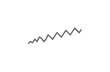
\begin{tikzpicture}[x=0.08em, y=0.08em, line width=0.4pt]
                \draw[FooterGray] (0,3) -- (1,4) -- (2,3.5) -- (3,5) -- (4,4) -- (5,6) -- (6,5.5) -- (7,4) -- (8,5) -- (9,7) -- (10,6) -- (11,5) -- (12,6.5) -- (13,8) -- (14,7) -- (15,6) -- (16,7.5) -- (17,9) -- (18,8) -- (19,7) -- (20,8.5) -- (21,10) -- (22,9) -- (23,8) -- (24,9.5);
            \end{tikzpicture}%
        }%
        \hskip0.5cm%
    }%
    \vskip6pt%
}

%=============================================================================
% PACHETE
%=============================================================================
\usepackage[utf8]{inputenc}
\usepackage[T1]{fontenc}
\usepackage{amsmath, amssymb, amsthm}
\usepackage{mathtools}
\usepackage{bm}
\usepackage{tikz}
\usetikzlibrary{arrows.meta, positioning, shapes, calc, decorations.pathreplacing, shadings}
\usepackage{booktabs}
\usepackage{multirow}
\usepackage{array}
\usepackage{graphicx}
\usepackage{hyperref}
\usepackage{colortbl}
\hypersetup{colorlinks=true, linkcolor=MainBlue, urlcolor=MainBlue}
\graphicspath{{../../logos/}{../../charts/}}
\hfuzz=2pt  % Suppress tiny overfull warnings (<2pt)

%=============================================================================
% COMANDA QUANTLET
%=============================================================================
\newcommand{\quantlet}[2]{%
    \hfill\href{#2}{%
        \raisebox{-0.15em}{\includegraphics[height=0.7em]{ql_logo.png}}%
        \textcolor{MainBlue}{\tiny\ #1}%
    }%
}

% Comandă pentru Quantlet sign sub grafice/tabele (format vechi, pentru compatibilitate)
\newcommand{\quantletsign}[1]{%
    \vspace{-2mm}%
    \hfill{\scriptsize\textcolor{MediumGray}{\faCode\ Quantlet: #1}}%
}

%=============================================================================
% MEDII PENTRU TEOREME
%=============================================================================
\theoremstyle{definition}
\setbeamertemplate{theorems}[numbered]
\newtheorem{defn}{Definiție}
\newtheorem{thm}{Teoremă}
\newtheorem{prop}{Propoziție}
\newtheorem{rmk}{Observație}

%=============================================================================
% COMENZI PERSONALIZATE
%=============================================================================
\newcommand{\E}{\mathbb{E}}
\newcommand{\Var}{\text{Var}}
\newcommand{\Cov}{\text{Cov}}
\newcommand{\Corr}{\text{Corr}}
\newcommand{\R}{\mathbb{R}}
\newcommand{\N}{\mathbb{N}}
\newcommand{\Z}{\mathbb{Z}}
\newcommand{\RMSE}{\text{RMSE}}
\newcommand{\MAE}{\text{MAE}}
\newcommand{\MAPE}{\text{MAPE}}

%=============================================================================
% PAGINĂ TITLU PERSONALIZATĂ
%=============================================================================
\defbeamertemplate*{title page}{hybrid}[1][]
{
    \vspace{0.2cm}
    % Logos row - top header (with clickable links)
    \begin{center}
        \href{https://www.ase.ro}{\includegraphics[height=1.0cm]{ase_logo.png}}\hspace{0.3cm}%
        \href{https://theida.net}{\includegraphics[height=1.0cm]{ida_logo.png}}\hspace{0.3cm}%
        \href{https://blockchain-research-center.com}{\includegraphics[height=1.0cm]{brc_logo.png}}\hspace{0.3cm}%
        \href{https://www.ai4efin.ase.ro}{\includegraphics[height=1.0cm]{ai4efin_logo.png}}\hspace{0.3cm}%
        \href{https://ipe.ro/new}{\includegraphics[height=1.0cm]{acad_logo.png}}\hspace{0.3cm}%
        \href{https://www.digital-finance-msca.com}{\includegraphics[height=1.0cm]{msca_logo.png}}%
    \end{center}

    \vspace{0.6cm}

    % Main title with Q logos on sides (with clickable links)
    \begin{center}
        \begin{minipage}{0.1\textwidth}
            \centering
            \href{https://quantlet.com}{\includegraphics[height=1.1cm]{ql_logo.png}}
        \end{minipage}%
        \begin{minipage}{0.78\textwidth}
            \centering
            {\LARGE\bfseries\usebeamercolor[fg]{title}\inserttitle}

            \vspace{0.3cm}

            {\usebeamerfont{subtitle}\usebeamercolor[fg]{title}\insertsubtitle}
        \end{minipage}%
        \begin{minipage}{0.1\textwidth}
            \centering
            \href{https://quantinar.com}{\includegraphics[height=1.1cm]{qr_logo.png}}
        \end{minipage}
    \end{center}

    \vspace{0.6cm}

    % Authors (left aligned)
    \hspace{0.5cm}{\usebeamerfont{author}\insertauthor}

    \vspace{0.3cm}

    % Institute/Affiliations (left aligned)
    \hspace{0.5cm}\begin{minipage}[t]{0.9\textwidth}
        \raggedright\small\insertinstitute
    \end{minipage}
}

%=============================================================================
% INFORMAȚII TITLU
%=============================================================================
\title[Analiza Seriilor de Timp]{Analiza și Prognoza seriilor de timp}
\subtitle{Capitolul 1: Introducere în Analiza seriilor de timp}
\author[D.T. Pele]{Daniel Traian PELE}
\institute{Academia de Studii Economice din București\\
IDA Institute Digital Assets\\
Blockchain Research Center\\
AI4EFin Artificial Intelligence for Energy Finance\\
Academia Română, Institutul de Prognoză Economică\\
MSCA Digital Finance}
\date{}

\begin{document}

% Title page (no header/footer)
{
\setbeamertemplate{headline}{}
\setbeamertemplate{footline}{}
\begin{frame}
    \titlepage
\end{frame}
}

%=============================================================================
% OBIECTIVELE CURSULUI
%=============================================================================
\begin{frame}{Obiective de învățare}
    \textbf{\large La sfârșitul acestui capitol, veți fi capabili să:}
    \vspace{0.15cm}
    \begin{enumerate}
        \item[\textcolor{MainBlue}{\textbf{1.}}] \textbf{Înțelegeți} procesele stochastice și realizările lor
        \vspace{0.08cm}
        \item[\textcolor{MainBlue}{\textbf{2.}}] \textbf{Definiți} staționaritatea strictă și slabă (de covarianță)
        \vspace{0.08cm}
        \item[\textcolor{MainBlue}{\textbf{3.}}] \textbf{Distingeți} între zgomot alb și mers aleatoriu
        \vspace{0.08cm}
        \item[\textcolor{MainBlue}{\textbf{4.}}] \textbf{Calculați} și interpretați funcția de autocorelație (ACF)
        \vspace{0.08cm}
        \item[\textcolor{MainBlue}{\textbf{5.}}] \textbf{Aplicați} funcția de autocorelație parțială (PACF)
        \vspace{0.08cm}
        \item[\textcolor{MainBlue}{\textbf{6.}}] \textbf{Utilizați} operatorul lag și diferențierea
        \vspace{0.08cm}
        \item[\textcolor{MainBlue}{\textbf{7.}}] \textbf{Efectuați} testul ADF pentru rădăcină unitate
        \vspace{0.08cm}
        \item[\textcolor{MainBlue}{\textbf{8.}}] \textbf{Aplicați} testul KPSS și interpretați rezultatele combinate
    \end{enumerate}
\end{frame}

%=============================================================================
% CUPRINS
%=============================================================================
\begin{frame}{Structura capitolului}
    \tableofcontents
\end{frame}

%=============================================================================
% SECȚIUNEA 1: PROCESE STOCHASTICE
%=============================================================================
\section{Procese Stochastice}

\begin{frame}{Proces stochastic: definiție}
    \begin{defn}[Proces Stochastic]
        Un \textbf{proces stochastic} este o colecție de variabile aleatoare indexate după timp:
        \[
            \{X_t(\omega) : t \in \mathcal{T}, \omega \in \Omega\}
        \]
        unde $\Omega$ este spațiul de selecție al rezultatelor posibile.
    \end{defn}

    \vspace{0.15cm}

    \textbf{Două perspective:}
    \begin{itemize}
        \item \textbf{$\omega$ fix}: O \textit{realizare} sau \textit{traiectorie de selecție} $\{X_t(\omega)\}_{t \in \mathcal{T}}$
        \item \textbf{$t$ fix}: O \textit{variabilă aleatoare} $X_t$ cu distribuția $F_t(x)$
    \end{itemize}

    \vspace{0.15cm}

    \textbf{Observație cheie:} O serie de timp pe care o observăm este \textbf{o realizare} a procesului stochastic subiacent. Folosim această singură realizare pentru a deduce proprietățile procesului.
\end{frame}

\begin{frame}{Proces stochastic: ilustrație vizuală}
    \begin{center}
        \includegraphics[width=0.9\textwidth]{ch1_def_stochastic.pdf}
    \end{center}
    \vspace{-0.2cm}
    \small Fiecare linie este o realizare diferită din același proces stochastic subiacent. Observăm doar o realizare dar vrem să înțelegem procesul.
\end{frame}

\begin{frame}{Momentele unui Proces Stochastic}
    \textbf{Primele două momente caracterizează proprietățile slabe:}

    \vspace{0.2cm}

    \textbf{Funcția de Medie:} \quad $\mu_t = \E[X_t]$

    \vspace{0.2cm}

    \textbf{Funcția de autocovarianță (ACVF):}
    \[
        \gamma(t, s) = \Cov(X_t, X_s) = \E[(X_t - \mu_t)(X_s - \mu_s)]
    \]

    \vspace{0.2cm}

    \textbf{Funcția de Autocorelație (ACF):}
    \[
        \rho(t, s) = \frac{\gamma(t, s)}{\sqrt{\Var(X_t) \cdot \Var(X_s)}}
    \]

    \vspace{0.2cm}

    \textbf{Proprietăți:} $\rho(t, s) \in [-1, 1]$ și $\rho(t, t) = 1$
\end{frame}

%=============================================================================
% SECȚIUNEA 4: STAȚIONARITATEA
%=============================================================================
\section{Staționaritatea}

\begin{frame}{De ce Contează Staționaritatea}
    \textbf{Staționaritatea} este o ipoteză fundamentală pentru analiza seriilor de timp:

    \vspace{0.15cm}

    \begin{columns}[T]
        \begin{column}{0.48\textwidth}
            \textbf{\textcolor{Crimson}{Fără Staționaritate:}}
            \begin{itemize}
                \item Media, varianța se schimbă în timp
                \item Trecutul poate să nu prezică viitorul
                \item Metodele standard eșuează
                \item Corelații false
            \end{itemize}
        \end{column}
        \begin{column}{0.48\textwidth}
            \textbf{\textcolor{Forest}{Cu Staționaritate:}}
            \begin{itemize}
                \item Proprietăți statistice constante
                \item Putem estima din o singură realizare
                \item Inferență validă posibilă
                \item Modelele sunt semnificative
            \end{itemize}
        \end{column}
    \end{columns}

    \vspace{0.2cm}

    \begin{alertblock}{Principiu Cheie}
        Majoritatea modelelor de serii de timp (ARMA, ARIMA, etc.) necesită staționaritate. Seriile nestaționare trebuie transformate (de ex., diferențiere) înainte de modelare.
    \end{alertblock}
\end{frame}

\begin{frame}{Staționar vs nestaționar: comparație Vizuală}
    \vspace{-0.3cm}
    \begin{center}
        \includegraphics[width=0.95\textwidth, height=0.62\textheight, keepaspectratio]{ch1_stationarity.pdf}
    \end{center}
    \vspace{-0.2cm}
    {\footnotesize
    \begin{itemize}
        \item \textbf{Staționar}: Medie și varianță constante -- fluctuează în jurul unui nivel fix
        \item \textbf{Nestaționar}: Media și/sau varianța se schimbă în timp
        \item Inspecția vizuală este primul pas; testele formale (ADF, KPSS) confirmă
    \end{itemize}
    }\quantlet{TSA\_ch1\_stationarity}{https://github.com/QuantLet/TSA/tree/main/ch1_stationarity}
\end{frame}

\begin{frame}{Staționaritate strictă}
    \begin{defn}[Staționaritate strictă (Puternică)]
        Un proces $\{X_t\}$ este \textbf{strict staționar} dacă pentru toți $k$, toți $t_1, \ldots, t_k$ și toți $h$:
        \[
            (X_{t_1}, X_{t_2}, \ldots, X_{t_k}) \stackrel{d}{=} (X_{t_1+h}, X_{t_2+h}, \ldots, X_{t_k+h})
        \]
    \end{defn}

    \vspace{0.15cm}

    \textbf{Interpretare:} Distribuția comună a oricărei colecții de observații este \textbf{invariantă la deplasări temporale}.

    \vspace{0.15cm}

    \textbf{Implicații:}
    \begin{itemize}
        \item Toate distribuțiile marginale $F_{X_t}(x)$ sunt identice
        \item $\E[X_t] = \mu$ (medie constantă)
        \item $\Var(X_t) = \sigma^2$ (varianță constantă)
        \item Distribuțiile comune depind doar de \textit{diferențele} temporale
    \end{itemize}

    \vspace{0.2cm}

    \textbf{Notă:} Staționaritatea strictă este o condiție puternică, adesea impractică de verificat.
\end{frame}

\begin{frame}{Staționaritate strictă: ilustrație vizuală}
    \begin{center}
        \includegraphics[width=0.95\textwidth]{ch1_def_strict_stationarity.pdf}
    \end{center}
    \vspace{-0.2cm}
    \small Staționar: oricare două ferestre au aceeași distribuție comună. Nestaționar: distribuția se schimbă în timp.
\end{frame}

\begin{frame}{Staționaritate slabă (de Covarianță)}
    \begin{defn}[Staționaritate slabă]
        Un proces $\{X_t\}$ este \textbf{slab staționar} (sau staționar de covarianță) dacă:
        \begin{enumerate}
            \item $\E[X_t] = \mu$ \quad (medie constantă)
            \item $\Var(X_t) = \sigma^2 < \infty$ \quad (varianță constantă, finită)
            \item $\Cov(X_t, X_{t+h}) = \gamma(h)$ \quad (covarianța depinde doar de lag-ul $h$)
        \end{enumerate}
    \end{defn}

    \vspace{0.15cm}

    \textbf{Proprietate cheie:} Autocovarianța este o funcție doar de lag:
    \[
        \gamma(h) = \Cov(X_t, X_{t+h}) = \E[(X_t - \mu)(X_{t+h} - \mu)]
    \]

    \vspace{0.2cm}

    \textbf{Funcția de autocorelație:}
    \[
        \rho(h) = \frac{\gamma(h)}{\gamma(0)} = \frac{\Cov(X_t, X_{t+h})}{\Var(X_t)}
    \]

    Notă: $\rho(0) = 1$ și $\rho(h) = \rho(-h)$ (simetrie)
\end{frame}

\begin{frame}{Staționaritate slabă: ilustrație vizuală}
    \begin{center}
        \includegraphics[width=0.95\textwidth]{ch1_def_weak_stationarity.pdf}
    \end{center}
    \vspace{-0.2cm}
    \small Stânga: medie și varianță constante. Dreapta: autocovarianța depinde doar de lag-ul $h$, nu de timpul $t$.
\end{frame}

\begin{frame}{Proprietățile funcției de autocovarianță}
    Pentru un proces slab staționar, ACVF $\gamma(h)$ satisface:

    \vspace{0.15cm}

    \begin{enumerate}
        \item \textbf{Simetrie:} $\gamma(h) = \gamma(-h)$

        \vspace{0.2cm}

        \item \textbf{Maxim la zero:} $|\gamma(h)| \leq \gamma(0)$

        \vspace{0.2cm}

        \item \textbf{Definit nenegativ}
    \end{enumerate}

    \vspace{0.15cm}

    \textbf{Implicație:} Nu orice funcție poate fi o funcție de autocovarianță.
\end{frame}

%=============================================================================
% SECȚIUNEA 5: ZGOMOT ALB ȘI MERS ALEATORIU
%=============================================================================
\section{Zgomot alb și Mers aleatoriu}

\begin{frame}{Procesul de Zgomot Alb}
    \begin{defn}[Zgomot Alb]
        Un proces $\{\varepsilon_t\}$ este \textbf{zgomot alb}, notat $\varepsilon_t \sim WN(0, \sigma^2)$, dacă:
        \begin{enumerate}
            \item $\E[\varepsilon_t] = 0$ pentru toți $t$
            \item $\Var(\varepsilon_t) = \sigma^2$ pentru toți $t$
            \item $\Cov(\varepsilon_t, \varepsilon_s) = 0$ pentru $t \neq s$
        \end{enumerate}
    \end{defn}

    \vspace{0.2cm}

    \textbf{ACF al Zgomotului Alb:}
    \[
        \rho(h) = \begin{cases}
            1 & \text{dacă } h = 0 \\
            0 & \text{dacă } h \neq 0
        \end{cases}
    \]

    \vspace{0.2cm}

    \textbf{Tipuri:}
    \begin{itemize}
        \item \textbf{Zgomot alb slab}: Necorelat (condițiile de mai sus)
        \item \textbf{Zgomot alb puternic}: Independent și identic distribuit (i.i.d.)
        \item \textbf{Zgomot alb Gaussian}: $\varepsilon_t \stackrel{iid}{\sim} N(0, \sigma^2)$
    \end{itemize}
\end{frame}

\begin{frame}{Zgomot alb vs mers aleatoriu: comparație}
    \vspace{-0.3cm}
    \begin{center}
        \includegraphics[width=0.95\textwidth, height=0.62\textheight, keepaspectratio]{ch1_wn_rw.pdf}
    \end{center}
    \vspace{-0.2cm}
    {\footnotesize
    \begin{itemize}
        \item \textbf{Zgomot alb}: Fluctuează în jurul lui zero -- staționar, varianță constantă
        \item \textbf{Mers aleatoriu}: Suma cumulativă a zgomotului alb -- rătăcește, nestaționar
        \item Mersul aleatoriu este cel mai simplu proces nestaționar (rădăcină unitate)
    \end{itemize}
    }\quantlet{TSA\_ch1\_wn\_rw}{https://github.com/QuantLet/TSA/tree/main/ch1_wn_rw}
\end{frame}

\begin{frame}{Zgomot alb: ilustrație vizuală}
    \begin{center}
        \includegraphics[width=0.95\textwidth]{ch1_def_white_noise.pdf}
    \end{center}
    \vspace{-0.2cm}
    \small Stânga: zgomotul alb fluctuează în jurul lui zero cu varianță constantă. Dreapta: ACF arată nicio autocorelație (toate zero după lag 0).
\end{frame}

\begin{frame}{Procesul de Mers aleatoriu}
    \textbf{Definiție:} $X_t = X_{t-1} + \varepsilon_t$ unde $\varepsilon_t \sim WN(0, \sigma^2)$, $X_0 = 0$

    \vspace{0.2cm}

    \textbf{Forma explicită:} $X_t = \sum_{i=1}^{t} \varepsilon_i$

    \vspace{0.15cm}

    \textbf{Proprietăți:}
    \begin{itemize}
        \item $\E[X_t] = 0$ (medie constantă)
        \item $\Var(X_t) = t\sigma^2$ (varianța crește în timp!)
        \item $\Cov(X_t, X_s) = \min(t, s) \cdot \sigma^2$
    \end{itemize}

    \vspace{0.15cm}

    \begin{alertblock}{Nestaționar!}
        Mersul aleatoriu \textbf{nu este staționar} deoarece varianța depinde de $t$.
    \end{alertblock}
\end{frame}

\begin{frame}{Mers aleatoriu: vizualizare}
    \begin{center}
        \includegraphics[width=0.95\textwidth, height=0.65\textheight, keepaspectratio]{random_walk.pdf}
    \end{center}
    \vspace{-0.2cm}
    \small \textbf{Stânga:} Traiectorii multiple divergă în timp. \textbf{Dreapta:} Varianța crește liniar: $\Var(X_t) = t\sigma^2$.
\end{frame}

\begin{frame}{Staționar vs nestaționar: comparație}
    \begin{center}
        \includegraphics[width=0.95\textwidth, height=0.65\textheight, keepaspectratio]{rw_vs_stationary.pdf}
    \end{center}
    \vspace{-0.2cm}
    \small\textbf{Diagnostic cheie:} ACF al procesului staționar scade rapid; ACF al mersului aleatoriu scade foarte lent.
\end{frame}

%=============================================================================
% SECȚIUNEA 6: ACF ȘI PACF
%=============================================================================
\section{Funcții de Autocorelație}

\begin{frame}{Funcția de autocorelație din eșantion}
    \textbf{ACF din eșantion la lag-ul $h$:}
    \[
        \hat{\rho}(h) = \frac{\sum_{t=1}^{T-h}(x_t - \bar{x})(x_{t+h} - \bar{x})}{\sum_{t=1}^{T}(x_t - \bar{x})^2}
    \]

    \vspace{0.15cm}

    \textbf{Proprietăți:}
    \begin{itemize}
        \item $\hat{\rho}(0) = 1$ întotdeauna
        \item $|\hat{\rho}(h)| \leq 1$
    \end{itemize}

    \vspace{0.15cm}

    \textbf{Test de semnificație:} Sub zgomot alb, $\hat{\rho}(h) \approx N(0, 1/T)$

    \vspace{0.2cm}

    \textbf{Limite 95\%:} $\pm 1.96/\sqrt{T}$
\end{frame}

\begin{frame}{Tipare ACF pentru diferite procese}
    \vspace{-0.3cm}
    \begin{center}
        \includegraphics[width=0.95\textwidth, height=0.62\textheight, keepaspectratio]{ch1_acf_examples.pdf}
    \end{center}
    \vspace{-0.2cm}
    {\footnotesize
    \begin{itemize}
        \item \textbf{Zgomot alb}: ACF scade la zero imediat (nicio dependență)
        \item \textbf{AR(1)}: ACF scade exponențial -- indică structură autoregresivă
        \item \textbf{Sezonier}: ACF arată vârfuri la lag-uri sezoniere (de ex., 12, 24 pentru lunar)
        \item \textbf{Mers aleatoriu}: ACF scade foarte lent -- semn de nestaționaritate
    \end{itemize}
    }\quantlet{TSA\_ch1\_acf\_examples}{https://github.com/QuantLet/TSA/tree/main/ch1_acf_examples}
\end{frame}

\begin{frame}{Funcția de autocorelație parțială (PACF)}
    \textbf{PACF} $\phi_{hh}$: Corelația dintre $X_t$ și $X_{t+h}$ după eliminarea efectului liniar al $X_{t+1}, \ldots, X_{t+h-1}$.

    \vspace{0.15cm}

    \textbf{Interpretare:}
    \begin{itemize}
        \item $\phi_{11} = \rho(1)$ (același ca ACF la lag 1)
        \item $\phi_{22} = $ corelația lui $X_t, X_{t+2}$ controlând pentru $X_{t+1}$
        \item Măsoară dependența \textit{directă} la lag-ul $h$
    \end{itemize}

    \vspace{0.15cm}

    \textbf{Aplicație cheie:} Identificarea ordinului AR
    \begin{itemize}
        \item Pentru AR($p$): PACF \textbf{se întrerupe} după lag-ul $p$
        \item Pentru MA($q$): ACF \textbf{se întrerupe} după lag-ul $q$
    \end{itemize}
\end{frame}

\begin{frame}{Tipare ACF și PACF}
    \begin{center}
        \includegraphics[width=0.95\textwidth, height=0.82\textheight, keepaspectratio]{acf_pacf_examples.pdf}
    \end{center}
\end{frame}

\begin{frame}{ACF teoretic pentru AR(1)}
    \begin{center}
        \includegraphics[width=0.95\textwidth, height=0.68\textheight, keepaspectratio]{acf_theoretical.pdf}
    \end{center}
    \vspace{-0.2cm}
    \small Pentru AR(1): $X_t = \phi X_{t-1} + \varepsilon_t$, ACF teoretic este $\rho(h) = \phi^h$.
\end{frame}

%=============================================================================
% SECȚIUNEA 7: OPERATORUL LAG ȘI DIFERENȚIEREA
%=============================================================================
\section{Operatorul lag și Diferențierea}

\begin{frame}{Operatorul lag}
    \begin{defn}[Operatorul lag]
        \textbf{Operatorul lag} (sau operatorul de întârziere) $L$ este definit prin:
        \[
            LX_t = X_{t-1}
        \]
    \end{defn}

    \vspace{0.2cm}

    \textbf{Proprietăți:}
    \begin{itemize}
        \item $L^k X_t = X_{t-k}$ (întârziere cu $k$ perioade)
        \item $L^0 = I$ (identitate)
        \item $(1 - \phi L)X_t = X_t - \phi X_{t-1}$
    \end{itemize}

    \vspace{0.2cm}

    \textbf{Exemple:}
    \begin{itemize}
        \item AR(1): $(1 - \phi L)X_t = \varepsilon_t$
        \item MA(1): $X_t = (1 + \theta L)\varepsilon_t$
        \item AR($p$): $(1 - \phi_1 L - \phi_2 L^2 - \cdots - \phi_p L^p)X_t = \varepsilon_t$
    \end{itemize}
\end{frame}

\begin{frame}{Operatorul lag: ilustrație vizuală}
    \begin{center}
        \includegraphics[width=0.9\textwidth]{ch1_def_lag_operator.pdf}
    \end{center}
    \vspace{-0.2cm}
    \small Operatorul lag $L$ deplasează fiecare observație înapoi cu o perioadă de timp: $LX_t = X_{t-1}$.
\end{frame}

\begin{frame}{Diferențierea}
    \textbf{Prima diferență:} $\Delta X_t = X_t - X_{t-1} = (1 - L)X_t$

    \vspace{0.15cm}

    \textbf{De ce diferențiem?}
    \begin{itemize}
        \item Elimină trendul și rădăcina unitate
        \item Mers aleatoriu: $\Delta X_t = \varepsilon_t$ (zgomot alb)
    \end{itemize}

    \vspace{0.15cm}

    \textbf{Proces integrat:} $X_t \sim I(d)$ dacă $\Delta^d X_t$ este staționar
    \begin{itemize}
        \item $I(0)$: Staționar (nu necesită diferențiere)
        \item $I(1)$: Necesită o diferențiere
        \item $I(2)$: Necesită două diferențieri
    \end{itemize}
\end{frame}

\begin{frame}{Efectul diferențierii: S\&P 500}
    \begin{center}
        \includegraphics[width=0.95\textwidth, height=0.82\textheight, keepaspectratio]{differencing_effect.pdf}
    \end{center}
\end{frame}

%=============================================================================
% SECȚIUNEA 8: TESTAREA STAȚIONARITĂȚII
%=============================================================================
\section{Testarea Staționarității}

\begin{frame}{Testul Augmented Dickey-Fuller (ADF)}
    \textbf{Model:} $\Delta X_t = \alpha + \gamma X_{t-1} + \sum_{i=1}^{p} \delta_i \Delta X_{t-i} + \varepsilon_t$

    \vspace{0.15cm}

    \begin{columns}[T]
        \begin{column}{0.48\textwidth}
            \textbf{Ipoteze:}
            \begin{itemize}
                \item $H_0$: $\gamma = 0$ (rădăcină unitate)
                \item $H_1$: $\gamma < 0$ (staționar)
            \end{itemize}
        \end{column}
        \begin{column}{0.48\textwidth}
            \textbf{Statistica de test:}
            \[
                \tau = \frac{\hat{\gamma}}{SE(\hat{\gamma})}
            \]
        \end{column}
    \end{columns}

    \vspace{0.15cm}

    \textbf{Decizie:}
    \begin{itemize}
        \item $\tau <$ valoare critică $\Rightarrow$ Respingem $H_0$ $\Rightarrow$ \textcolor{Forest}{Staționar}
        \item $\tau \geq$ valoare critică $\Rightarrow$ \textcolor{Crimson}{Nestaționar}
    \end{itemize}

    \vspace{0.2cm}
    \small Valori critice: distribuția Dickey-Fuller (nu normală)
\end{frame}

\begin{frame}{Testul KPSS}
    \textbf{Model:} $X_t = \xi t + r_t + \varepsilon_t$ unde $r_t = r_{t-1} + u_t$

    \vspace{0.2cm}

    \begin{columns}[T]
        \begin{column}{0.48\textwidth}
            \textbf{Ipoteze (opuse față de ADF):}
            \begin{itemize}
                \item $H_0$: $\sigma_u^2 = 0$ (staționar)
                \item $H_1$: $\sigma_u^2 > 0$ (rădăcină unitate)
            \end{itemize}
        \end{column}
        \begin{column}{0.48\textwidth}
            \textbf{Statistica de test:}
            \[
                LM = \frac{\sum_{t=1}^{T} S_t^2}{T^2 \hat{\sigma}^2}
            \]
            {\small unde $S_t = \sum_{i=1}^{t} \hat{e}_i$}
        \end{column}
    \end{columns}

    \vspace{0.2cm}

    \textbf{Decizie:}
    \begin{itemize}
        \item $LM >$ valoare critică $\Rightarrow$ Respingem $H_0$ $\Rightarrow$ \textcolor{Crimson}{Nestaționar}
        \item $LM \leq$ valoare critică $\Rightarrow$ \textcolor{Forest}{Staționar}
    \end{itemize}

    \vspace{0.1cm}
    \small \textbf{Notă:} KPSS complementează ADF---folosiți ambele pentru concluzii robuste.
\end{frame}

\begin{frame}{Folosirea ADF și KPSS împreună}
    \textbf{Testare confirmatorie} pentru concluzii robuste:

    \vspace{0.15cm}

    \begin{center}
    \begin{tabular}{lccl}
        \toprule
        \textbf{ADF} & \textbf{KPSS} & \textbf{Concluzie} \\
        \midrule
        Respingem $H_0$ & Nu respingem $H_0$ & \textcolor{Forest}{Staționar} \\
        Nu respingem $H_0$ & Respingem $H_0$ & \textcolor{Crimson}{Rădăcină Unitate} \\
        Respingem $H_0$ & Respingem $H_0$ & Neconcludent \\
        Nu respingem $H_0$ & Nu respingem $H_0$ & Neconcludent \\
        \bottomrule
    \end{tabular}
    \end{center}

    \vspace{0.15cm}

    \textbf{Flux de lucru recomandat:}
    \begin{enumerate}
        \item Rulați testul ADF (nulă = rădăcină unitate)
        \item Rulați testul KPSS (nulă = staționar)
        \item Dacă rezultatele coincid, procedați cu încredere
        \item Dacă neconcludent, considerați teste alternative (PP, DF-GLS)
    \end{enumerate}
\end{frame}

\begin{frame}{Testul ADF: vizualizare cu S\&P 500}
    \begin{center}
        \includegraphics[width=0.95\textwidth, height=0.82\textheight, keepaspectratio]{adf_test_visualization.pdf}
    \end{center}
\end{frame}

%=============================================================================
% SECȚIUNEA 9: APLICAȚIE PE DATE REALE
%=============================================================================
\section{Aplicație pe Date Financiare}

\begin{frame}{Analiza S\&P 500: prezentare generală}
    \begin{center}
        \includegraphics[width=0.95\textwidth, height=0.82\textheight, keepaspectratio]{sp500_analysis.pdf}
    \end{center}
\end{frame}

\begin{frame}{Fapte stilizate ale Randamentelor Financiare}
    \begin{center}
        \includegraphics[width=0.95\textwidth, height=0.48\textheight, keepaspectratio]{returns_distribution.pdf}
    \end{center}

    \vspace{0.1cm}
    \begin{columns}[T]
        \begin{column}{0.48\textwidth}
            \textbf{Proprietăți observate:}
            \begin{itemize}
                \item Asimetrie negativă (coadă stângă)
                \item Kurtoză excesivă ($\gg 3$)
                \item Cozi groase (heavy tails)
            \end{itemize}
        \end{column}
        \begin{column}{0.48\textwidth}
            \textbf{Implicații:}
            \begin{itemize}
                \item Distribuția normală inadecvată
                \item Evenimente extreme mai probabile
                \item Necesită distribuție Student-t sau similară
            \end{itemize}
        \end{column}
    \end{columns}
\end{frame}

\begin{frame}{Gruparea volatilității}
    \begin{columns}[T]
        \column{0.35\textwidth}
        \begin{alertblock}{Fapt Stilizat}
            Randamentele mari (pozitive sau negative) tind să fie urmate de randamente mari. Această \textbf{grupare a volatilității} motivează modelele ARCH/GARCH (capitolele viitoare).
        \end{alertblock}
        \column{0.63\textwidth}
        \vspace{-0.3cm}
        \begin{center}
            \includegraphics[width=\textwidth, height=0.78\textheight, keepaspectratio]{volatility_clustering.pdf}
        \end{center}
    \end{columns}
\end{frame}

%=============================================================================
% SECȚIUNEA 10: REZUMAT
%=============================================================================
\section{Rezumat}

\begin{frame}{Concluzii cheie}
    \small
    \begin{enumerate}
        \item \textbf{Proces stochastic} = colecție de variabile aleatoare indexate după timp
        \vspace{0.08cm}
        \item \textbf{Realizare} = o traiectorie observată din procesul stochastic subiacent
        \vspace{0.08cm}
        \item \textbf{Staționaritate slabă}: Medie constantă, varianță constantă, autocovarianță depinde doar de lag
        \vspace{0.08cm}
        \item \textbf{Zgomot alb}: Proces necorelat cu medie zero și varianță constantă
        \vspace{0.08cm}
        \item \textbf{Mers aleatoriu}: Suma cumulativă a zgomotului alb --- nestaționar
        \vspace{0.08cm}
        \item \textbf{ACF/PACF}: Instrumente esențiale pentru identificarea structurii de dependență
        \vspace{0.08cm}
        \item \textbf{Operatorul lag}: $LX_t = X_{t-1}$; diferențiere: $\Delta X_t = X_t - X_{t-1}$
        \vspace{0.08cm}
        \item \textbf{Testul ADF}: $H_0$: rădăcină unitate (nestaționar)
        \vspace{0.08cm}
        \item \textbf{Testul KPSS}: $H_0$: staționar --- folosiți împreună cu ADF pentru concluzii robuste
    \end{enumerate}
\end{frame}

\begin{frame}{Formule importante I}
    \begin{block}{Staționaritate slabă}
        \begin{itemize}
            \item $\E[X_t] = \mu$ (medie constantă)
            \item $\Var(X_t) = \sigma^2 < \infty$ (varianță constantă)
            \item $\Cov(X_t, X_{t+h}) = \gamma(h)$ (depinde doar de lag)
        \end{itemize}
    \end{block}

    \begin{block}{Zgomot alb: $\varepsilon_t \sim WN(0, \sigma^2)$}
        $\E[\varepsilon_t] = 0$, \quad $\Var(\varepsilon_t) = \sigma^2$, \quad $\Cov(\varepsilon_t, \varepsilon_s) = 0$ pentru $t \neq s$
    \end{block}

    \begin{block}{Mers aleatoriu}
        $X_t = X_{t-1} + \varepsilon_t$ \quad $\Rightarrow$ \quad $\Var(X_t) = t\sigma^2$ (nestaționar!)
    \end{block}
\end{frame}

\begin{frame}{Formule importante II}
    \begin{block}{Autocovarianță și Autocorelație}
        $\gamma(h) = \Cov(X_t, X_{t+h})$ \qquad $\rho(h) = \frac{\gamma(h)}{\gamma(0)}$
    \end{block}

    \begin{block}{ACF din eșantion}
        $\hat{\rho}(h) = \frac{\sum_{t=1}^{T-h}(x_t - \bar{x})(x_{t+h} - \bar{x})}{\sum_{t=1}^{T}(x_t - \bar{x})^2}$
    \end{block}

    \begin{block}{Operatorul lag și Diferențierea}
        $LX_t = X_{t-1}$ \qquad $\Delta X_t = (1-L)X_t = X_t - X_{t-1}$
    \end{block}

    \begin{block}{Test ADF}
        $H_0$: $\gamma = 0$ (rădăcină unitate) \quad vs \quad $H_1$: $\gamma < 0$ (staționar)
    \end{block}
\end{frame}

\begin{frame}{Previzualizare capitolul următor}
    \textbf{Capitolul 2: Modele ARMA}

    \vspace{0.2cm}

    \begin{itemize}
        \item Modele Autoregresive (AR)
        \item Modele de Medie Mobilă (MA)
        \item Modele ARMA combinate
        \item Identificarea modelului folosind ACF/PACF
        \item Estimarea parametrilor
        \item Diagnosticarea modelului
        \item Prognoza
    \end{itemize}
\end{frame}

%=============================================================================
% SECȚIUNEA: QUIZ
%=============================================================================
\section{Quiz}

\begin{frame}{Întrebarea quiz 1}
    \begin{alertblock}{Întrebare}
        O serie de timp $Y_t$ arată mișcare ascendentă de-a lungul anilor plus tipare repetitive în fiecare trimestru. Ce componente sunt prezente?
    \end{alertblock}

    \vspace{0.3cm}

    \begin{enumerate}[(A)]
        \item Doar trend
        \item Doar sezonalitate
        \item Trend și Sezonalitate
        \item Doar zgomot aleatoriu
    \end{enumerate}
\end{frame}

\begin{frame}{Întrebarea quiz 1: Răspuns}
    \begin{columns}[T]
        \column{0.35\textwidth}
        \begin{exampleblock}{Răspuns Corect: (C) Trend și Sezonalitate}
            Mișcare ascendentă = Trend; Tipare trimestriale = Sezonalitate (s=4)
        \end{exampleblock}
        \column{0.63\textwidth}
        \vspace{-0.3cm}
        \begin{center}
            \includegraphics[width=\textwidth, height=0.78\textheight, keepaspectratio]{ch1_quiz1_components.pdf}
        \end{center}
    \end{columns}
\end{frame}

\begin{frame}{Întrebarea quiz 2}
    \begin{alertblock}{Întrebare}
        Care dintre următoarele este o caracteristică a unei serii de timp staționare?
    \end{alertblock}

    \vspace{0.3cm}

    \begin{enumerate}[(A)]
        \item Media se schimbă în timp
        \begin{itemize}
            \item Estimatorul punctual: $\bar{x} = \frac{1}{n}\sum_{i=1}^n x_i$
            \item Proprietăți: nedeplasare, consistență
        \end{itemize}
        \item Varianța crește în timp
        \begin{itemize}
            \item Măsoară dispersia în jurul mediei
            \item Estimator: $s^2 = \frac{1}{n-1}\sum_{i=1}^n (x_i - \bar{x})^2$
        \end{itemize}
        \item Medie și varianță constante în timp
        \item Conține o componentă de trend
    \end{enumerate}
\end{frame}

\begin{frame}{Întrebarea quiz 2: Răspuns}
    \begin{columns}[T]
        \column{0.35\textwidth}
        \begin{exampleblock}{Răspuns Corect: (C) Medie și varianță constante în timp}
            Staționaritatea necesită: medie constantă, varianță constantă și autocovarianța depinde doar de lag.
        \end{exampleblock}
        \column{0.63\textwidth}
        \vspace{-0.3cm}
        \begin{center}
            \includegraphics[width=\textwidth, height=0.78\textheight, keepaspectratio]{ch1_quiz2_stationarity.pdf}
        \end{center}
    \end{columns}
\end{frame}

\begin{frame}{Întrebarea quiz 3}
    \begin{alertblock}{Întrebare}
        Pentru un proces de zgomot alb, cum arată ACF la lag-uri $k > 0$?
    \end{alertblock}

    \vspace{0.3cm}

    \begin{enumerate}[(A)]
        \item Descreștere exponențială
        \item Toate valorile semnificative și pozitive
        \item Toate valorile aproximativ zero (în interiorul benzilor de încredere)
        \item Alternare pozitiv și negativ
    \end{enumerate}
\end{frame}

\begin{frame}{Întrebarea quiz 3: Răspuns}
    \begin{columns}[T]
        \column{0.35\textwidth}
        \begin{exampleblock}{Răspuns Corect: (C) Aproximativ zero în interiorul benzilor de încredere}
            Zgomotul alb nu are autocorelație: $\rho_k = 0$ pentru toți $k \neq 0$.
        \end{exampleblock}
        \column{0.63\textwidth}
        \vspace{-0.3cm}
        \begin{center}
            \includegraphics[width=\textwidth, height=0.78\textheight, keepaspectratio]{ch1_quiz3_acf.pdf}
        \end{center}
    \end{columns}
\end{frame}

\begin{frame}{Întrebarea quiz 4}
    \begin{alertblock}{Întrebare}
        Care este diferența cheie între zgomotul alb și mersul aleatoriu?
    \end{alertblock}

    \vspace{0.3cm}

    \begin{enumerate}[(A)]
        \item Zgomotul alb are trend, mersul aleatoriu nu
        \item Mersul aleatoriu este suma cumulativă a zgomotului alb
        \item Ambele sunt procese staționare
        \item Zgomotul alb are varianță mai mare
    \end{enumerate}
\end{frame}

\begin{frame}{Întrebarea quiz 4: Răspuns}
    \begin{columns}[T]
        \column{0.35\textwidth}
        \begin{exampleblock}{Răspuns Corect: (B) Mers aleatoriu = suma cumulativă a zgomotului alb}
            $Y_t = Y_{t-1} + \varepsilon_t = \sum_{i=1}^t \varepsilon_i$ unde $\varepsilon_t$ este zgomot alb.
        \end{exampleblock}
        \column{0.63\textwidth}
        \vspace{-0.3cm}
        \begin{center}
            \includegraphics[width=\textwidth, height=0.78\textheight, keepaspectratio]{ch1_quiz4_wn_rw.pdf}
        \end{center}
    \end{columns}
\end{frame}

\begin{frame}{Întrebarea quiz 5}
    \begin{alertblock}{Întrebare}
        Care metrică de eroare a prognozei este cea mai sensibilă la erori mari (valori aberante)?
    \end{alertblock}

    \vspace{0.3cm}

    \begin{enumerate}[(A)]
        \item MAE (Eroarea Medie Absolută)
        \item RMSE (Rădăcina Erorii Medii Pătratice)
        \item MAPE (Eroarea Medie Absolută Procentuală)
        \item Toate sunt la fel de sensibile
    \end{enumerate}
\end{frame}

\begin{frame}{Întrebarea quiz 5: Răspuns}
    \begin{columns}[T]
        \column{0.35\textwidth}
        \begin{exampleblock}{Răspuns Corect: (B) RMSE}
            RMSE ridică la pătrat erorile, deci erorile mari au impact disproporționat: $\sqrt{\frac{1}{n}\sum e_t^2}$
        \end{exampleblock}
        \column{0.63\textwidth}
        \vspace{-0.3cm}
        \begin{center}
            \includegraphics[width=\textwidth, height=0.78\textheight, keepaspectratio]{ch1_quiz5_forecast_errors.pdf}
        \end{center}
    \end{columns}
\end{frame}

\begin{frame}{Întrebarea quiz 6}
    \begin{alertblock}{Întrebare}
        Când ar trebui să folosiți descompunerea multiplicativă în loc de cea aditivă?
    \end{alertblock}

    \vspace{0.3cm}

    \begin{enumerate}[(A)]
        \item Când seria nu are trend
        \item Când amplitudinea sezonieră este constantă
        \item Când amplitudinea sezonieră crește odată cu nivelul seriei
        \item Când seria este staționară
    \end{enumerate}
\end{frame}

\begin{frame}{Întrebarea quiz 6: Răspuns}
    \begin{columns}[T]
        \column{0.35\textwidth}
        \begin{exampleblock}{Răspuns Corect: (C) Amplitudinea sezonieră crește odată cu nivelul}
            multiplicativă: $Y_t = T_t \times S_t \times \varepsilon_t$ --- oscilațiile sezoniere proporționale cu trendul.
        \end{exampleblock}
        \column{0.63\textwidth}
        \vspace{-0.3cm}
        \begin{center}
            \includegraphics[width=\textwidth, height=0.78\textheight, keepaspectratio]{ch1_quiz6_decomposition.pdf}
        \end{center}
    \end{columns}
\end{frame}

%=============================================================================
\section{Studiu de Caz: PIB România}
%=============================================================================

\begin{frame}{Studiu de Caz: PIB Trimestrial România}
    \begin{center}
        \includegraphics[width=0.95\textwidth, height=0.75\textheight, keepaspectratio]{ch1_case_gdp_raw.pdf}
    \end{center}

    \begin{itemize}
        \item \textbf{Date}: PIB trimestrial România, 2010--2023 (sursa: INS/Eurostat)
        \item \textbf{Observații}: Trend crescător, sezonalitate trimestrială, șoc COVID-19 în 2020
    \end{itemize}
\end{frame}

\begin{frame}{Descompunerea seriei PIB}
    \begin{center}
        \includegraphics[width=0.95\textwidth, height=0.78\textheight, keepaspectratio]{ch1_case_gdp_decomposition.pdf}
    \end{center}
\end{frame}

\begin{frame}{Interpretarea componentelor}
    \begin{columns}[T]
        \begin{column}{0.5\textwidth}
            \begin{block}{Componente Identificate}
                \begin{itemize}
                    \item \textbf{Trend}: Creștere economică susținută
                    \item \textbf{Sezonalitate}: Pattern trimestrial regulat (Q4 > Q1)
                    \item \textbf{Reziduu}: Include șocul COVID-19 din 2020
                \end{itemize}
            \end{block}
        \end{column}
        \begin{column}{0.5\textwidth}
            \begin{alertblock}{Lecții Învățate}
                \begin{itemize}
                    \item Descompunerea ajută la înțelegerea structurii datelor
                    \item Șocurile externe (COVID) apar în componenta reziduală
                    \item Sezonalitatea trebuie modelată explicit
                \end{itemize}
            \end{alertblock}
        \end{column}
    \end{columns}

    \vspace{0.5cm}

    \begin{exampleblock}{Următorii Pași}
        În capitolele următoare vom învăța să modelăm fiecare componentă: ARIMA pentru trend, SARIMA pentru sezonalitate.
    \end{exampleblock}
\end{frame}

%=============================================================================
\section{Referințe}
%=============================================================================



%=============================================================================
% SURSE DE DATE
%=============================================================================
\begin{frame}{Surse de Date}
    \begin{block}{Date Reale Utilizate în Acest Capitol}
        \begin{itemize}
            \item \textbf{Pasageri Aviație}: Set de date clasic Box-Jenkins, 1949--1960
            \item \textbf{S\&P 500}: Yahoo Finance (SPY), date istorice
            \item \textbf{Pete Solare}: Set de date Statsmodels, observații lunare
        \end{itemize}
    \end{block}

    \begin{block}{Software și Instrumente}
        \begin{itemize}
            \item \textbf{Python}: statsmodels, pandas, matplotlib, yfinance
            \item \textbf{R}: pachetele forecast, tseries
            \item \textbf{Surse de Date}: Yahoo Finance, FRED Economic Data
        \end{itemize}
    \end{block}
\end{frame}

\begin{frame}{}
    \centering
    \Huge\textcolor{MainBlue}{Vă Mulțumesc!}

    \vspace{1cm}

    \Large Întrebări?

    \vspace{0.8cm}

    \normalsize
    \textit{Grafice generate folosind Python (statsmodels, matplotlib)}

    \vspace{0.3cm}

    Materiale curs disponibile la: \url{https://github.com/danpele/Time-Series-Analysis}
\end{frame}


%=============================================================================
% BIBLIOGRAFIE
%=============================================================================
\begin{frame}{Bibliografie I}
    \begin{block}{Manuale fundamentale}
        {\small
        \begin{itemize}
            \item Hyndman, R.J., \& Athanasopoulos, G. (2021). \textit{Forecasting: Principles and Practice}, 3rd ed., OTexts.
            \item Shumway, R.H., \& Stoffer, D.S. (2017). \textit{Time Series Analysis and Its Applications}, 4th ed., Springer.
            \item Brockwell, P.J., \& Davis, R.A. (2016). \textit{Introduction to Time Series and Forecasting}, 3rd ed., Springer.
        \end{itemize}
        }
    \end{block}

    \begin{exampleblock}{Serii de timp financiare}
        {\small
        \begin{itemize}
            \item Tsay, R.S. (2010). \textit{Analysis of Financial Time Series}, 3rd ed., Wiley.
            \item Franke, J., Härdle, W.K., \& Hafner, C.M. (2019). \textit{Statistics of Financial Markets}, 4th ed., Springer.
        \end{itemize}
        }
    \end{exampleblock}
\end{frame}

\begin{frame}{Bibliografie II}
    \begin{block}{Abordari moderne si Machine Learning}
        {\small
        \begin{itemize}
            \item Nielsen, A. (2019). \textit{Practical Time Series Analysis}, O'Reilly Media.
            \item Petropoulos, F., et al. (2022). \textit{Forecasting: Theory and Practice}, International Journal of Forecasting.
            \item Makridakis, S., Spiliotis, E., \& Assimakopoulos, V. (2020). The M4 Competition, International Journal of Forecasting.
        \end{itemize}
        }
    \end{block}

    \begin{exampleblock}{Resurse online si cod}
        {\small
        \begin{itemize}
            \item \textbf{Quantlet}: \url{https://quantlet.com} --- Repository de cod pentru statistica
            \item \textbf{Quantinar}: \url{https://quantinar.com} --- Platforma de invatare metode cantitative
            \item \textbf{GitHub TSA}: \url{https://github.com/QuantLet/TSA} --- Cod Python pentru acest curs
        \end{itemize}
        }
    \end{exampleblock}
\end{frame}

\end{document}
